%%%%%%%%%%%%%%%%%%%%%%%%%%%%%%%%%%%%%%%%%%%%%%%%%%%%%%%%%%%%%%%%%%%%%%
%%                     Truth
%%%%%%%%%%%%%%%%%%%%%%%%%%%%%%%%%%%%%%%%%%%%%%%%%%%%%%%%%%%%%%%%%%%%%%
%\color{green}
\subsection{\glyph{Truth} }\label{sec:truth}

\glyph{Truth} is the arc used to represent the connection of a boolean operator to another. For instance, A \glyph{and} \glyph{not} B.

\begin{description}
 \glyphSboTerm To be determined.
 \glyphOrigin Any logical operator (section~\ref{sec:logic}).
 \glyphTarget Any logical operator (section~\ref{sec:logic}).
 \item[end-points]\mbox{}\\ No particular symbol is used to represent at the extremities of truth arc.
 \end{description}

\begin{center}
\scalebox{0.5}{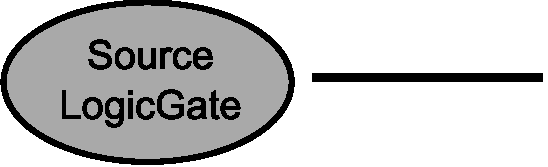
\includegraphics{images/truth}}
\end{center}
\normalcolor
